%\section{Background and Overview}
%\label{sec:gsgx:background}

%\subsection{\intel{} \sgx{} Enclaves}
%\label{sec:graphene:background:sgx}

%\begin{figure}[t!]
%\centering
%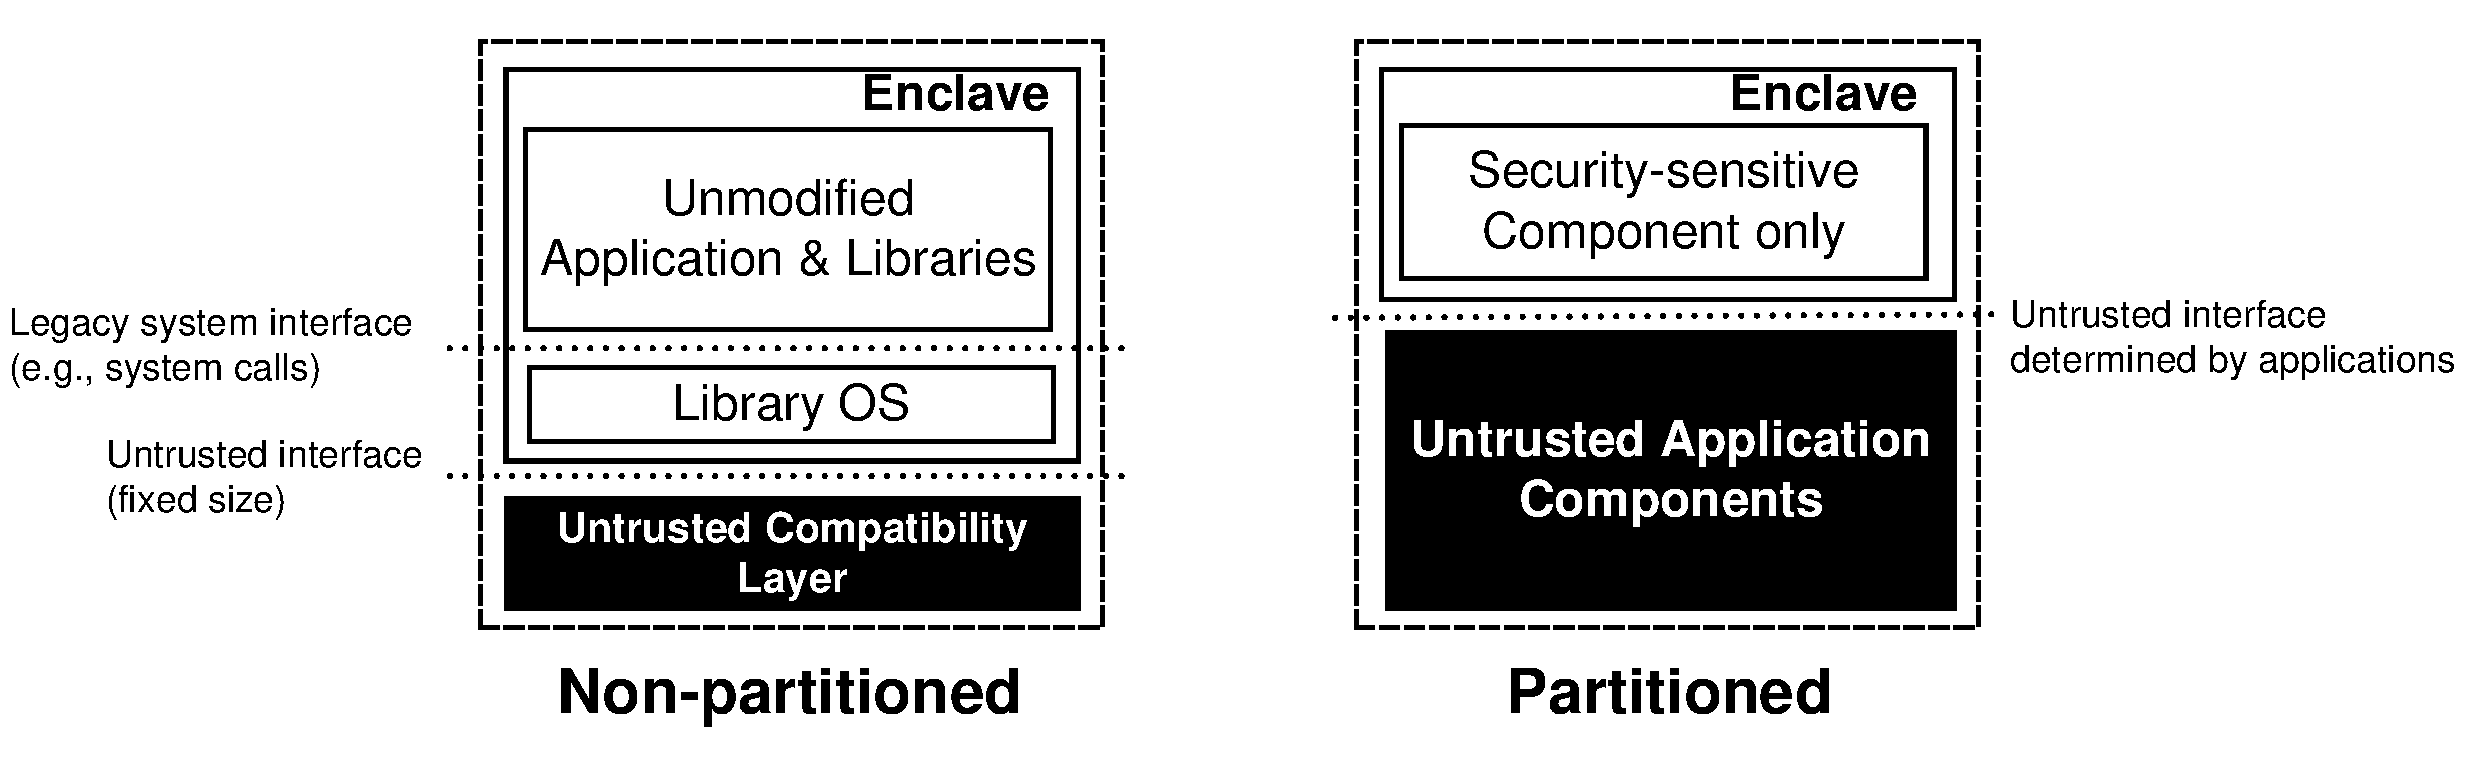
\includegraphics[width=5in]{graphene-sgx/figures/libosvssdk.pdf}
%\footnotesize
%\vspace{-0.3in}
%\caption[Comparison between libOS-based model and partitioned model for Intel SGX]
%{Comparison between libOS-based model (e.g., \haven{} and \sysname{})
%and SDK-based (SDK for \sgx{}) model for migrating applications in enclaves.
%Green (light) boxes are trusted components and red (dark) boxes are untrusted.
%The libOS-based model often yields a larger TCB in the enclave,
%while the SDK-based model requires developers to be responsible of
%securing the enclave on the untrusted interface.}
%\label{fig:libosvssdk}
%\end{figure}

\intel{} \sgx{} (Software Guard Extension)
is a set of new x86/x86\_64 instructions
introduced in the latest \intel{} \skylake{} processors,
to create, interface and attest
an isolated memory region (\term{enclave}) inside applications' virtual memory.
\sgx{} guarantee any data in an enclave
stay encrypted in the DRAMs, using a secret key derived from
the application's cryptographic measurements.
The secret data store in the enclave memory
can only be accessed within the code inside the enclave,
and the code must be signed by the developers' private key.
The use cases of \sgx{} mostly involve an enclave
retrieving a signed attestation from the \intel{} processor,
to exchange provisioning of information from trusted remote servers.
The purpose is equivalent to
expanding the execution from remote servers
to untrusted hosts,
to securely harness resources such as CPU cycles and DRAMs.

\sgx{} is an appealing tool for protecting small, highly sensitive execution, 
against malicious or compromised OSes, hypervisors, or even hardware peripheral.
For instance, \cite{hoekstra13sgx} show how SGX can be used
to build a trusted path from a video chat application to a GPU and network card, which maintains confidentiality and integrity of the
video stream, even if the OS is compromised.
Similarly, because DRAM contents are encrypted, SGX can resist attacks such as cold-boot attacks~\citep{halderman09coldboot} or 
malicious peripheral devices~\citep{hudson15thunderstrike}.

\paragraph{A Partitioned Usage Model.}
To secure an application with \sgx{},
the common usage model requires the developers to partition the application into two parts:
the trusted code will run the sensitive execution in the enclave,
while the untrusted code will load and interact with the trusted code.
Even if the trusted code only contains the simplest the logic,
the untrusted code is still needed to pass the input and output of the execution.

The interaction between the trusted and untrusted code is through an \term{untrusted interface}.
An untrusted interface is often defined by the developers, and contains a set of logical entry and exit points of the enclave.
However, an enclave will only have exactly one hardware entry point and one hardware exit point.
The control transfer from the hardware entry point to the logical entry points
is based on the operation code passed as an argument at enclave entry.

With the partitioned usage model,
the developers can minimize the TCB of enclave at their best effort,
and define the behavior of the enclave that can only be triggered by the untrusted interface.
The process of partitioning can prevent unpredicted behaviors in the enclave,
which may compromise the security of the enclave.
The untrusted and trusted code must explicitly call for enclave entry or exit
at the fixed sites in the application.

%\intel{} \sgx{} ({\it Software Guard Extensions})
%are a set of new x86/x64 instructions
%introduced in the \intel{} Skylake processor family.
%Using \sgx{}, an 
%application can designate part of its virtual memory as an {\em enclave}.
%The CPU guarantees that the contents of the enclave never leave the CPU package unencrypted.
%The CPU also measures the integrity of a binary loaded into the enclave, and offers remote attestation,
%similar to a TPM~\citep{TPM}.


%%% create a protected memory region, called an {\em enclave}, inside it's virtual memory,
%%% where it can load its security sensitive data with hardware-enforced isolation from the untrusted OS. 
%%% The processor with \sgx{}
%%% guarantees that any data loaded in enclave
%%% stays encrypted in the DRAM, by using a secret key deterministically derived from the application's cryptographic measurement and the CPU secret. 



% \sgx{} provides useful building blocks for secure applications, but does not
%absolve the programmer of all responsibility for reasoning about end-to-end security.
%Bugs in the application or supporting libraries can still disclose sensitive data from an enclave,
%and porting code into SGX can be subtle.
%
%Fundamentally, this argues for writing enclave code in higher-level languages
%(e.g., \java{}) that provide important 
%safety properties, such as memory and type safety, that reduce or eliminate common vulnerabilities.
%Ideally, one would formally verify security properties of enclave code~\citep{moat}; this verification is significantly aided by using 
%higher-level languages amenable to formal reasoning.  Verification is significantly harder
%with C/C++ or assembly languages.

%One must note that \sgx{} only promises the integrity of application binaries
%initially loaded in enclaves.
%The gap between integrity of binaries and complete security has to be filled
%by ones who develop and approve the applications.
%More specifically, the clients are responsible of
%testing whether the applications contain any vulnerabilities
%that lead to information leak.
%To minimize the risk of leaving any flaws in the applications unintentionally,
%developers often tend to cut down the trusted computing base (TCB)
%of the applications. With smaller TCB, clients who launched the enclaves
%can more easily reason about the thoroughness of securing the execution.

%To achieve smaller TCB, the software development kit of \sgx{}
%intends to encourage developers to partition the applications and
%keep only security sensitive components in the enclaves.
%Such an intention is exactly contradicted by the trust model of \haven{},
%which must trust the loaded application as a whole.
%Except for the cases in which the whole applications must be secured,
%\haven{} actually downgrades the trustworthiness of enclaves.
%Figure~\ref{fig:gsgx:libosvssdk} shows the comparison of the two models.

\paragraph{Using A Library OS.}
 
The partitioned usage model restricts the risk of the isolated execution being compromised,
but requires the developers to be familiar with
the mechanism of enclave entry and exit,
and always bear the security of the isolated execution in mind.
For developers that are not expert to architecture and security issues,
pursuing the partitioned model may need significant efforts.   

\term{Haven}\citep{baumann14haven} is the first to show a non-partitioned usage model,
to load a native application with its supporting library
into the enclave.
The non-partitioned model allows application to be run in the enclave as it is, with minimal or no porting effort.
To support the non-partitioned model, the primary requirement is to support the system APIs called by the native application.
\haven{} uses \drawbridge{} \libos{}~\citep{porter11drawbridge}
to handle all the system API calls.

In low level, the non-partitioned model still requires partitioning, but the binary to be partitioned is the \libos{} itself.
More precisely, \drawbridge{} \pal{} is the component that is partitioned,
and rest of the \libos{}, alone with the application,
can be dynamically loaded into the enclave after the enclave starts.
The partitioned \drawbridge{} \pal{} interacts with a \libos{}-specific untrusted interface,
which is the only trusted interface needed to be defined,
and will never be extended no matter which application is loaded.
